% vim: ts=2 sw=2 et tw=78:

\section{Method of Characteristics}

The method of charactersitics can be used to solve Cauchy problems with first
order quasilinear PDEs.

\subsection{General Case}

Suppose we have an $u(x,y)$ and let $x$ and $y$ be parametrized by a new
variable $t$, i.e. $x(t)$ and $y(t)$. Then if we take the derivative by the
chain rule:
\[
  \frac{d}{dt} u(x,y) = \frac{\partial u}{\partial x} \frac{dx}{dt}
    + \frac{\partial u}{\partial y} \frac{dy}{dt}.
\]
By comparing this to the general form we see that if we let
\[
  a(x,y,u,t) = \frac{dx}{dt}, \quad
  b(x,y,u,t) = \frac{dy}{dt},
\]
we obtain the left side of the general PDE of the Cauchy problem
\eqref{eqn:cauchy-2d}. Considering the right side we also have that $du/dt =
c$. Solving this system of ODEs for the functions $x(t)$, $y(t)$ and $u(t)$ is
equivalent to solving the PDE. Each ODE will yield an expression in $t$ and
each will have an integration constant. The solution to the PDE can only
depend on these integration constant which are found using the initial datum.

\begin{figure}
  \centering
  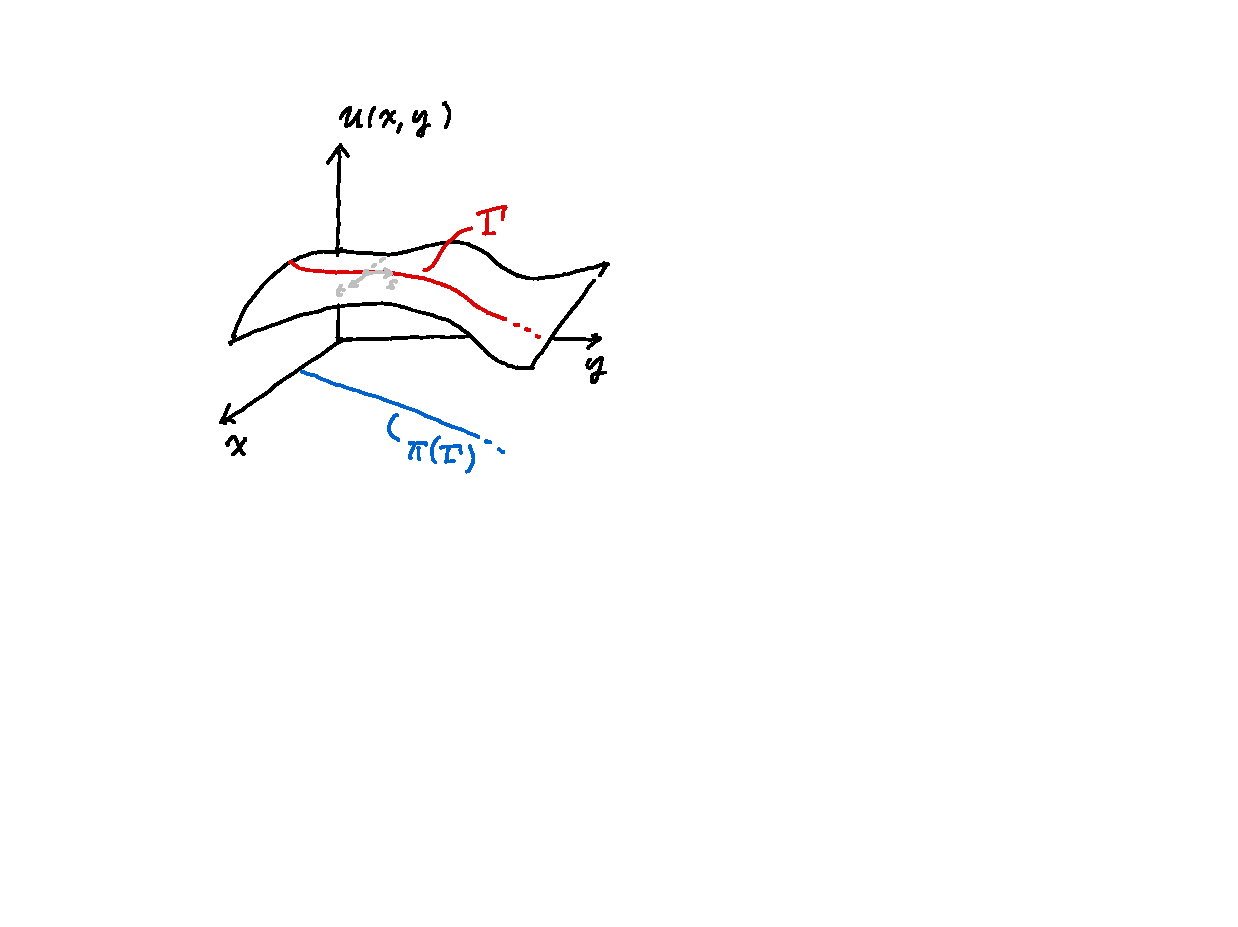
\includegraphics[
    width=.9\linewidth,
    trim=80 200 280 20, clip
  ]{figures/parametrization}
  \caption{
    Parametrization of the initial curve $\Gamma$ and its projection on the
    domain $\pi(\Gamma)$.
  }
\end{figure}

We parametrize the initial datum as a parametric curve $\Gamma$ with a
variable $s$, i.e.
\[
  \Gamma = \left\{
    \bigr( (x_0(s), y_0(s), u_0(s) \bigl) : s \in \mathbb{R}
  \right\}.
\]
For example if the initial curve is given as $u(x, 0) = x^2$, a good
parametrization is $\Gamma = \{ (s, 0, s^2) \}$. Then, these parametrization
are the initial values for the system of ODEs:
\[
  x(0) = x_0(s), \quad
  y(0) = y_0(s), \quad
  u(0) = u_0(s).
\]

Thus at the end of this process we have a solution $u$ to the PDE which is a
function of $(s, t)$; a local coordinate system. To conclude, we need to go
back to $(x,y)$, so we must invert the map to find $(s, t) \to (x(s,t),
y(s,t))$. This inversion is not always possible, to check whether the map is
(locally) invertible we use the \emph{transversality condition}.
\begin{thm}[Transversality condition]
  If the determinant of the Jacobian of a 2D Cauchy problem
  \[
    \det\begin{bmatrix}
      \partial_t x & \partial_t y \\
      \partial_s x_0 & \partial_s y_0
    \end{bmatrix}
    =
    \det\begin{bmatrix}
      a & b \\ \partial_s x_0 & \partial_s y_0
    \end{bmatrix}
    \neq 0,
  \]
  then there is a unique solution.
\end{thm}


\subsection{Special Cases}

If in \eqref{eqn:cauchy-2d} both $a$ and $b$ do \emph{not} depend on $u$ and
the PDE is homogeneous ($c = 0$) we can skip the parametrization. The PDE can
be rewritten using the dot product as
\[
  \begin{bmatrix} a(x,y) & b(x,y) \end{bmatrix}
    \cdot \nabla u(x,y) = 0,
\]
which is a directional derivative. With this interpretation we are saying that
$u$ must be constant along a curve defined by $a$ and $b$, which is equivalent
to stating that the slope must be given by
\[
  \frac{dy}{dx} = \frac{b(x,y)}{a(x,y)}.
\]
By solving this ODE we find the charactestic curves of $u$, one for each value
of the integration constant $k$. Thus the PDE has a general solution of the
form
\[
  u(x,y) = f(k(x,y)),
\]
and to find a particular solution one just needs to use the inital datum to
choose an appropriate $f$.
